In this section we present the results derived from the measurements of the peak bolometric luminosity and the trends observed with other parameters for the SNe in our low-reddening sample. We also extend the analysis to the complete sample of objects with a measured second maximum.


\begin{table*}
\caption{$L_{max}$ measurements for low reddening SNIa with a measured $t_2$. }

\begin{center}
\begin{tabular}{llccccrrr}
\hline
SN  & $L_{max}(\cdot e^{43} erg s^{-1})$ & $e_{L}$  & $M_{Ni}-Arn (M_{\odot})$  & $M_{Ni}-Arn (M_{\odot})$ (fixed rise)  & $M_{Ni}-DDC (M_{\odot})$\\% & $E(B-V)_{MW}$ & u-band lum \\
\hline
%SN2001ba & 1.18 & 0.15 & 0.58 & 0.59 & 	0.57 \\
SN2002dj & 1.25 & 0.26 & 0.59 & 0.63 & 0.61 \\
SN2002fk & 1.42 & 0.23 & 0.68 & 0.71 & 0.76 \\
SN2005M & 1.37 & 0.08 & 0.70 & 0.69 & 0.71 \\
SN2005am & 1.1 & 0.2 & 0.47 & 0.55 & 0.52 \\
SN2005el & 0.91	& 0.11 & 0.40 & 0.46   & 0.44 	\\	
SN2005eq & 1.32 & 0.2 & 0.67 & 0.66 & 0.67 \\
SN2005hc & 1.36 & 0.2 & 0.69 & 0.68 & 0.71 \\
SN2005iq & 1.07 & 0.11 & 0.48 & 0.54 & 0.51 \\
SN2005ki & 1.03 & 0.27 & 0.45 & 0.51 & 0.49 \\
SN2006bh & 0.86 & 0.15 & 0.37 & 0.43 & 0.40 \\
SN2007bd & 1.22 & 0.13 & 0.55	  & 0.61 & 0.59	\\
SN2007on & 0.6 & 0.09 & 0.24 & 0.30 & 0.28 \\
SN2008R & 0.53 & 0.1 & 0.21 & 0.26 & 0.25 \\
SN2008bc & 1.24 & 0.19 & 0.60 & 0.62 & 0.63 \\
SN2008gp & 1.29 & 0.14 & 0.62 & 0.65 & 0.64 \\
SN2008hv & 1.08 & 0.13 & 0.48 & 0.54 & 0.52 \\
SN2008ia & 1.13 & 0.14 & 0.50 & 0.57 & 0.55 \\
SN2011fe & 1.1 & 0.15 & 0.50 & 0.55 & 0.52 \\
\hline
\end{tabular}
\label{tab:mni}
\end{center}
\end{table*}

\subsection{Correlation between $L_{max}$ and $t_2$ }

In figure ~\ref{fig:nit2}, we find that there is a very strong correlation between $t_2$ and $M_{^{56}Ni}$ in the $Y$ and $J$ bands with $r$ values of 
0.80, 0.88. A much weaker trend is observed in the $H$ band with $r \sim$ 0.60. This is reflected in the ratio of the slope to the slope error in equation \eqref{eq:lin_t2}

\begin{table}
\caption{Values of the coefficients for correlations between $L_{max}$ and $t_2$ in the individual filters}
\begin{center}
\begin{tabular}{llcc}
\hline
Filter & $a_i $ & $b_i $	 \\
\hline
Y    &	0.043($\pm$0.005)  &	-0.100($\pm$0.133)	\\
J    & 	0.040($\pm$0.004)  &	-0.047($\pm$0.118)		\\
H    & 	0.036($\pm$0.009)  &	 0.256($\pm$0.222)		\\
\hline
\end{tabular}
\end{center}
\label{tab:coeff}
\end{table}


In the $Y$ and $J$ band, a strong correlation suggests that objects with more Ni produced show later second maxima. 
\begin{equation}
\label{eq:lmt2}
L_{max}=a_i \cdot t_2(i) + b_i
\end{equation}

From Table ~\ref{tab:coeff} and figure \ref{fig:nit2}, we can see that the constraints on the slope for the best fit relation in the $H$ band are weak. Hence, for further analyses, we do not use the $H$ band.

Equation \eqref{eq:lmt2} relates $t_2$ to the bolometric luminosity. The coefficients for the linear fit and the errors on the estimates are given in Table ~\ref{tab:coeff}. 
%Equations \eqref{eq:ly,eq:lj,eq:lh} relate the timing of the second maximum to the peak bolometric luminosity by combining equation \eqref{eq:eni} with equation \eqref{eq:y,eq:j,eq:h}. We can see that the relation is dependent on the rise time of the SN and the $\alpha$ parameter which encodes the deviation from Arnett's rule.

%From the equations it is evident that the timing of the second maximum in $H$ doesn't provide stringent constraints on the bolometric peak luminosity.
\subsection{Low galactic reddening sample}
In our sample, we selected objects with a host galaxy extinction $<$ 0.1 mag. For some of these objects, the galactic extinction is $>$ 0.1 mag. In order to see whether these objects influence the strength of the correlation, we evaluate the correlation coefficients for a sample without the high galactic reddening objects.
 As a result, 7 objects with $E(B-V)_{host}<$0.1 but total E(B-V) $\geq$ 0.1 are removed. We do not find a substantial decrease in the correlation coefficients in the $YJH$ bands, which are 0.76, 0.83, 0.60 respectively. Since we know the reddening law in the MW with high certainty, we can correct the bolometric light curves for the absorption from the MW dust. Thus, for further analysis we do not truncate the sample from the original low reddening objects in Table ~\ref{tab:lr}




\subsection{Deriving $M_{^{56}Ni}$ from $L_{max}$}
\label{ssec-derni}
In the sections above, we have found a strong correlation between $L_{max}$ and $t_2$ in the $Y$ and $J$ bands. 
%From this correlation we have derived a value for the peak bolometric luminosity of a sample of 5 highly reddened supernovae, which we have summarised in Table ~\ref{tab:red}.

Since our final aim is to derive a value of the $^{56}Ni$ mass for objects which have a measured value of $t_2$, we present the different methods to derive $M_{^{56}Ni}$ from the peak bolometric luminosity.

In figure \ref{fig:nicomp}, we plot the distributions of the $M_{^{56}Ni}$ from the different methods.
\subsubsection{Arnett's rule with a variable rise time}
Arnett's rule states that the luminosity of the SN at peak is given by the instantaneous rate of energy deposition from radioactive decays inside the expanding ejecta. 
This is summarized in equation \eqref{eq:lm-eni}. 
\begin{equation}
L_{max}=\alpha E_{Ni} (t_R)
\end{equation}

Where $E_{Ni}$ is the input from $^{56}$Ni decay at maximum, $t_R$ is the rise time and $\alpha$ accounts for deviations from Arnett's Rule.

\begin{equation}
\label{eq:eni}
E_{Ni} (1 M_{\odot})= 6.45  \cdot 10^{43} e^{-t_R/8.8} + 1.45  \cdot  10^{43} e^{-t_R/111.3}
\end{equation}

For estimates using different rise times, we follow the relation in \citet{G2011}
\begin{equation}
t_{R, B}=17.5 - 5(\Delta m_{15} - 1.1)
\end{equation}
and  
\begin{equation}
t_{R, Bol}=t_{R, B}+ (t_{max, bol} -t_{max, B})
\end{equation}
which implies 

\begin{multline}
L_{max}=\alpha \cdot (6.45  \cdot  10^{43} e^{-(t_{R, bol}/8.8}) + \\ 1.45  \cdot  10^{43} e^{-t_{R,bol}/111.3})  \cdot(M_{Ni}/M_{\odot})
\end{multline}

substituting the relation derived between $L_{max}$ and $t_2$ (equation \eqref{eq:lmt2}) we get a relation between $t_2$ and $M_{^{56}Ni}$

\begin{equation}
\label{eq:nit2}
M_{^{56}Ni}= \frac{a_i \cdot t_2(i) + b_i}{\alpha \cdot E_{Ni}(t_2(i))} 
\end{equation}

From equation \eqref{eq:nit2}, we can see that the relation between $M_{^{56}Ni}$ and $t_2$ is non-linear.  

 
\subsubsection{Arnett's rule with a fixed rise time}
For this method of deriving $M_{^{56}Ni}$ from $L_{max}$, we use a fixed rise time of 19 days, as in \citet{Stritzinger2006}. Similar to their analysis, we propagate an uncertainty of $\pm$ 3 days 
\begin{equation}
\label{eq:arn}
L_{max}=(2.0 \pm 0.3) \cdot 10^{43} (M_{^{56}Ni}/M_{\odot}) erg s^{-1}
\end{equation}

For deriving equation \eqref{eq:arn} we need to use a specific value of $\alpha$. In previous studies \citep[eg.][]{Stritzinger2006,Mazzali2007}, the authors use $\alpha$=1. This value is very close to the self consisent models of \citet{Arnett1982} and is also the mean values for the models of \citet{Hoeflich1995}. Hence, in our study, we use $\alpha$=1.

From the DDC models, we calculate the ratio of decay energy to the bolometric luminosity (which is the $\alpha$ value) for the different $M_{^{56}Ni}$ input values. We find that the values have a mean of 1.03 with a $\sigma$ of 0.07. We find that these values are consistent with the simplifying assumption that $\alpha$=1.
  
\begin{figure}
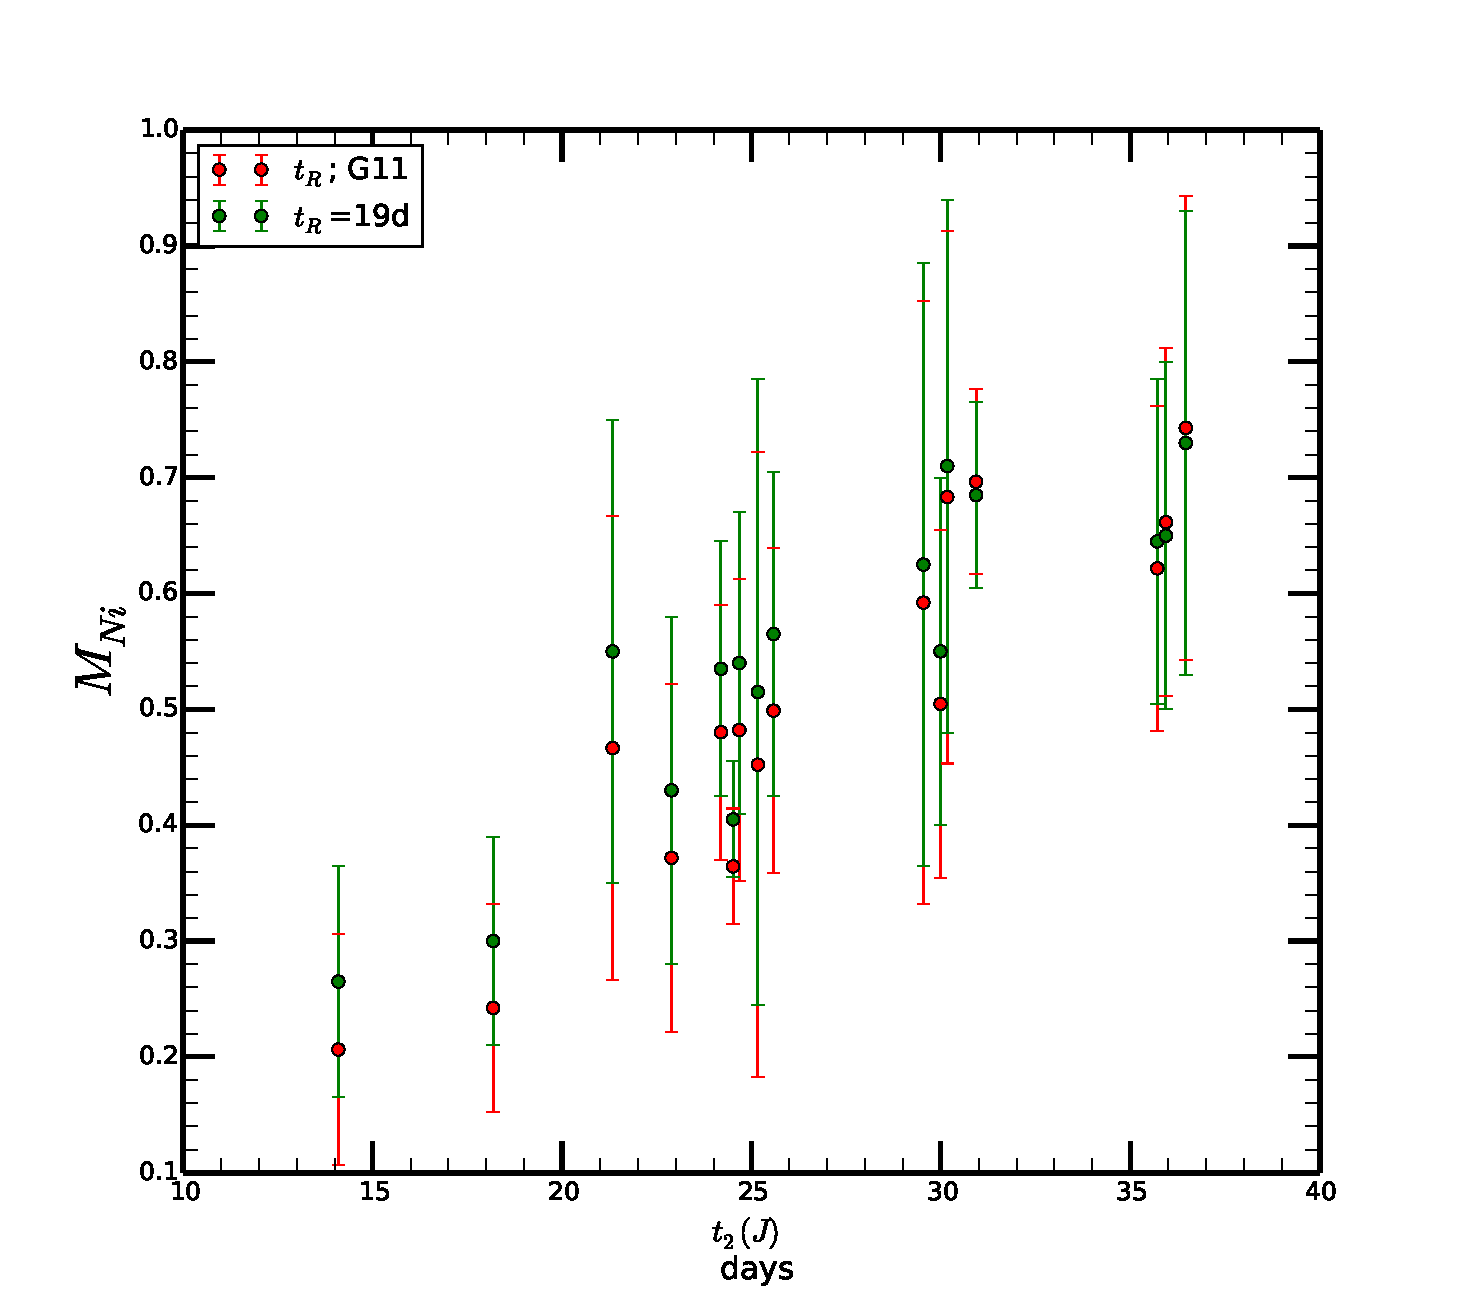
\includegraphics[width=.5\textwidth, trim= 0 30 0 30]{../plot_rel/comp_tr_nit2.pdf}
\caption{Comparison of the $M_{^{56}Ni}$ versus $t_2$ relations for using Arnett's rule with variable (\emph{red circles}) and fixed (\emph{green circles}) rise time. }
\end{figure}

%----------------------------------%

\subsubsection{Interpolating using DDC models}
Another possible method for deriving   $M_{^{56}Ni}$ values from $L_{max}$ is by interpolating the relation found from theoretical models between these two quantities. In our analysis, we use the DDC models from \citet{Blondin2013} as another method of obtaining $M_{^{56}Ni}$.

For objects without NIR coverage, these models can be used to calculate the $M_{^{56}Ni}$-$L_{max}$ relationship for a set of optical-only filters (eg. SN2004gu only has $BVRI$ coverage near maximum). 
This method, therefore, has the advantage of being able to derive $M_{^{56}Ni}$ values for objects with missing passbands without an additional correction term applied to the $L_{max}$. However, in order to keep the samples uniform across the different methods, we only use the objects with complete coverage from $u$ ot $H$ bands. 

%----------%

\begin{figure}
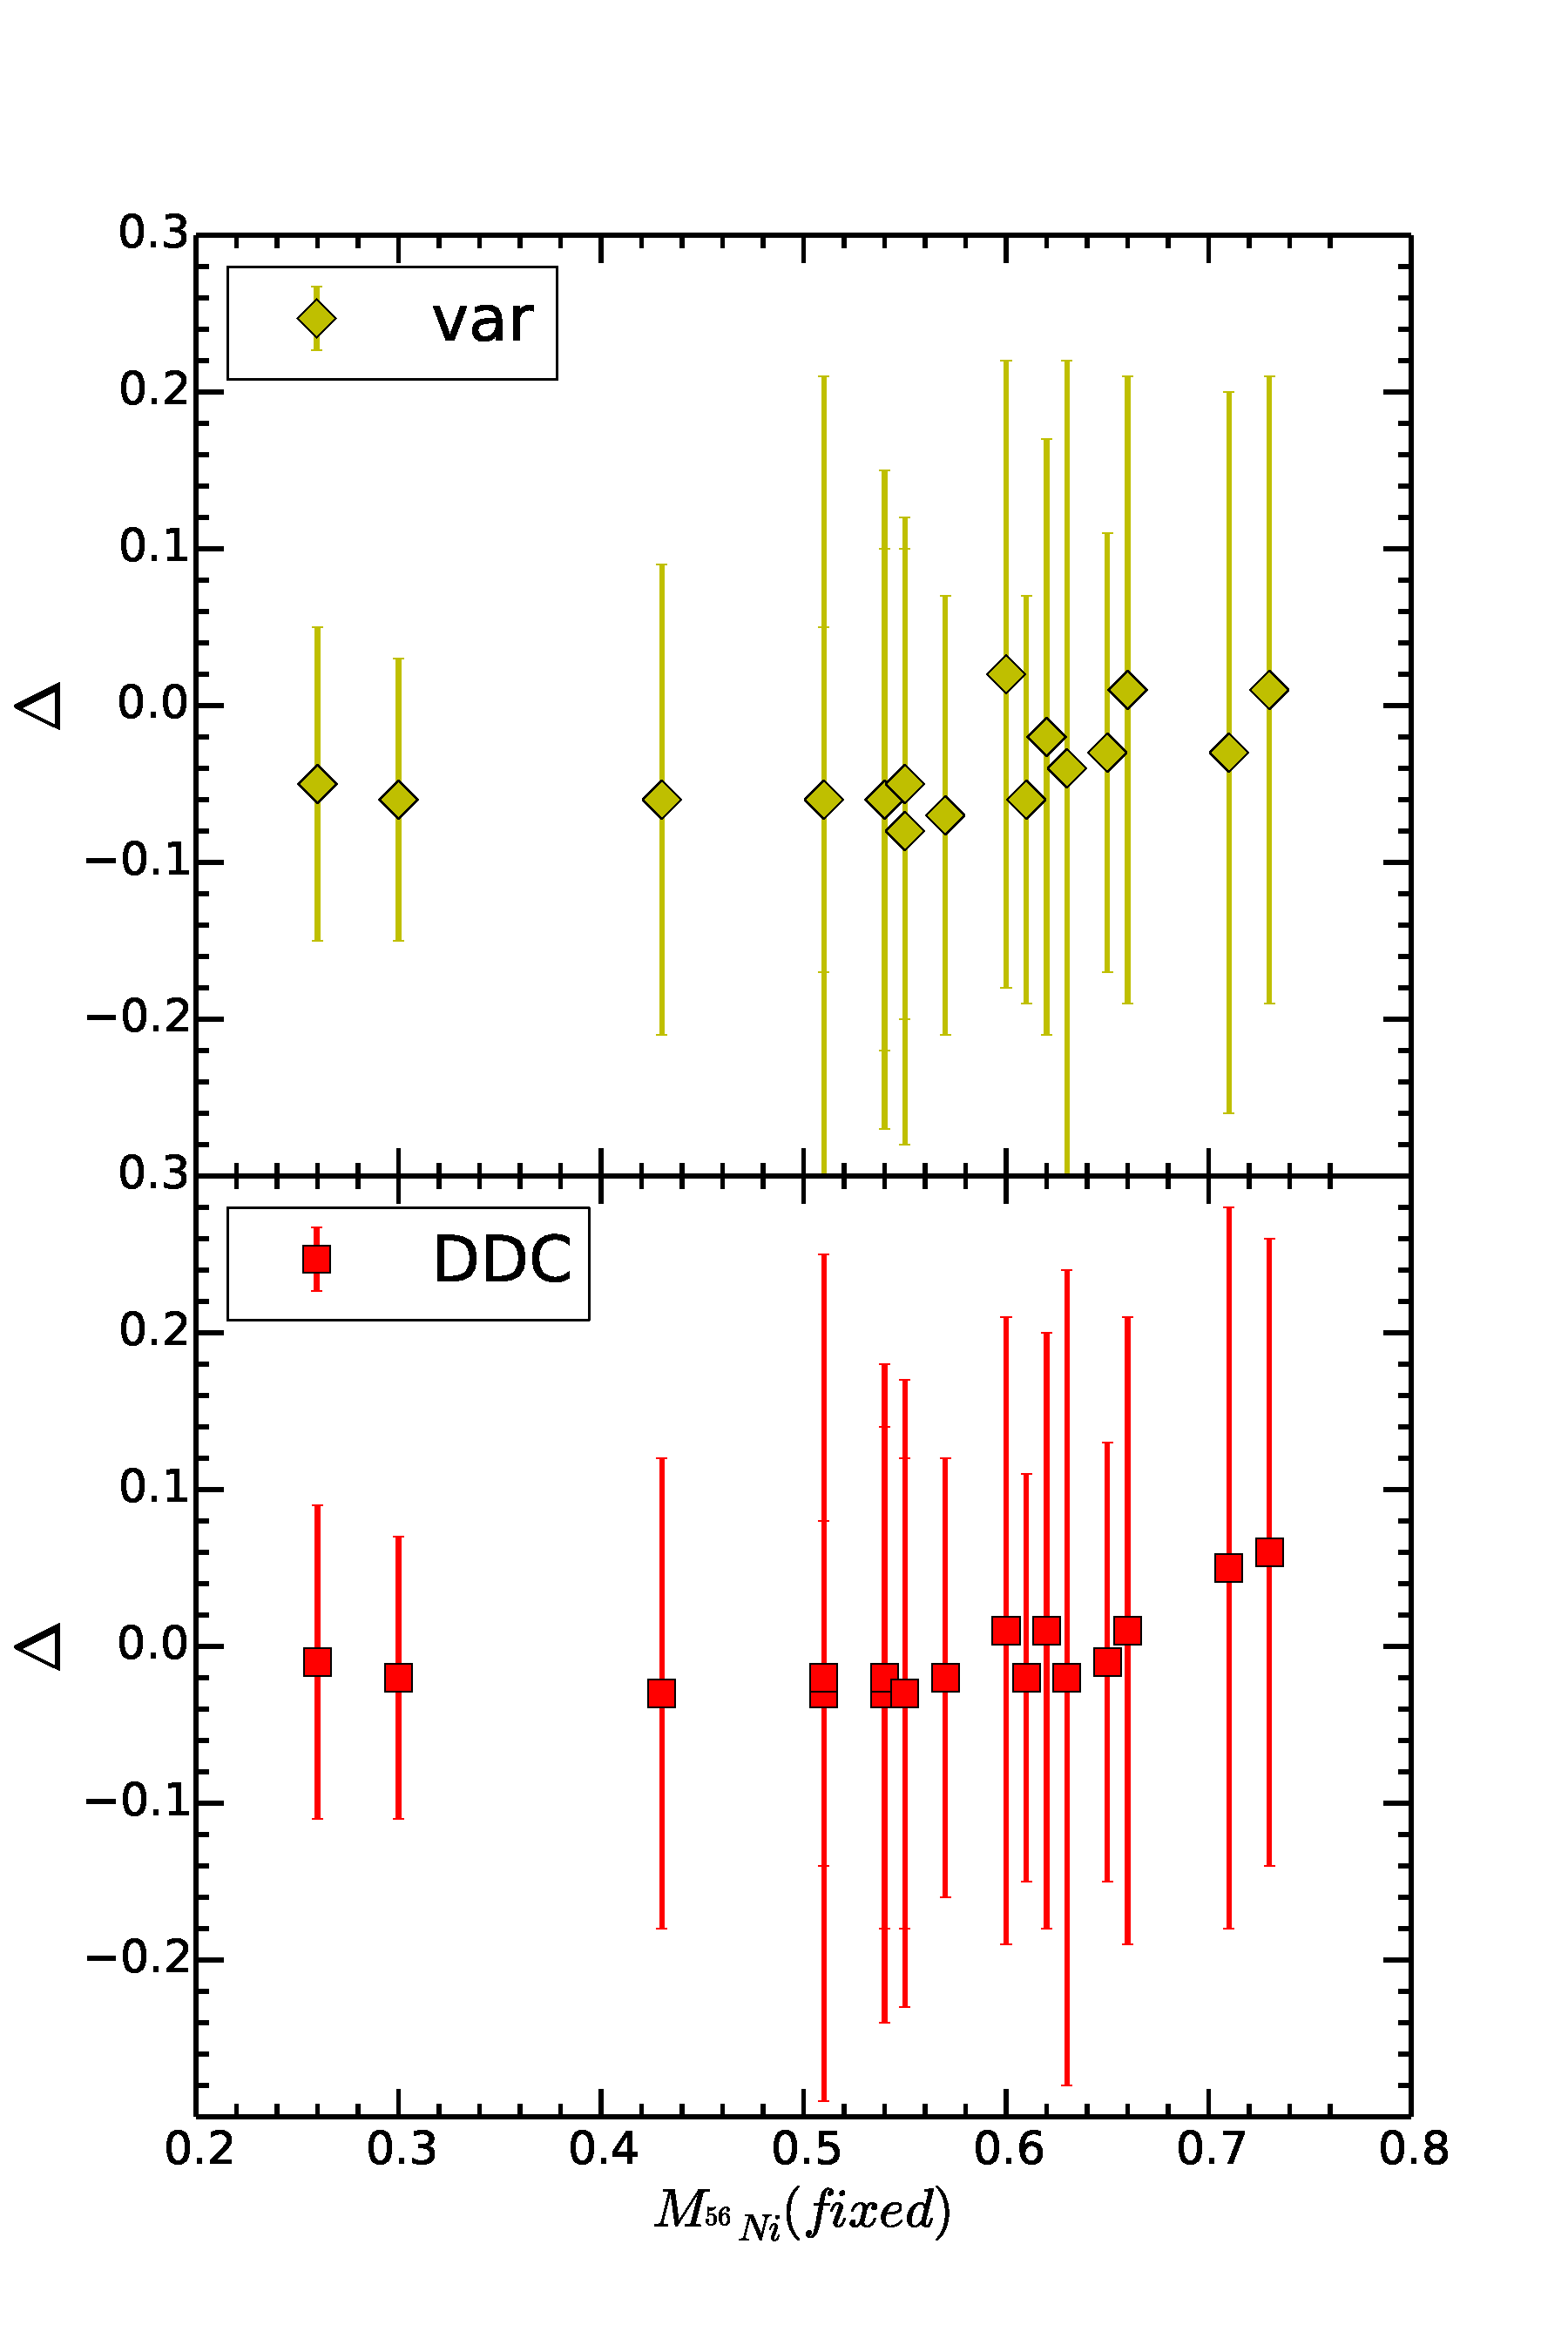
\includegraphics[width=.5\textwidth, trim= 0 30 0 30]{../plot_rel/dif_ni_comp.pdf}
\caption{\emph{Top}: The difference between the values estimated using a fixed rise time with Arnett's rule and the DDC models is plotted against the estimates from Arnett's rule with fixed rise time. \emph{Bottom}: The difference between values estimated using a fixed rise time with Arnett's rule and a variable rise time plotted against the estimates from Arnett's rule with fixed rise time. From the two panels we can see that the difference in the individual measurements are much smaller than the errors from a given method}
\label{fig:difarn}
\end{figure}

%---------------% 

\begin{figure}
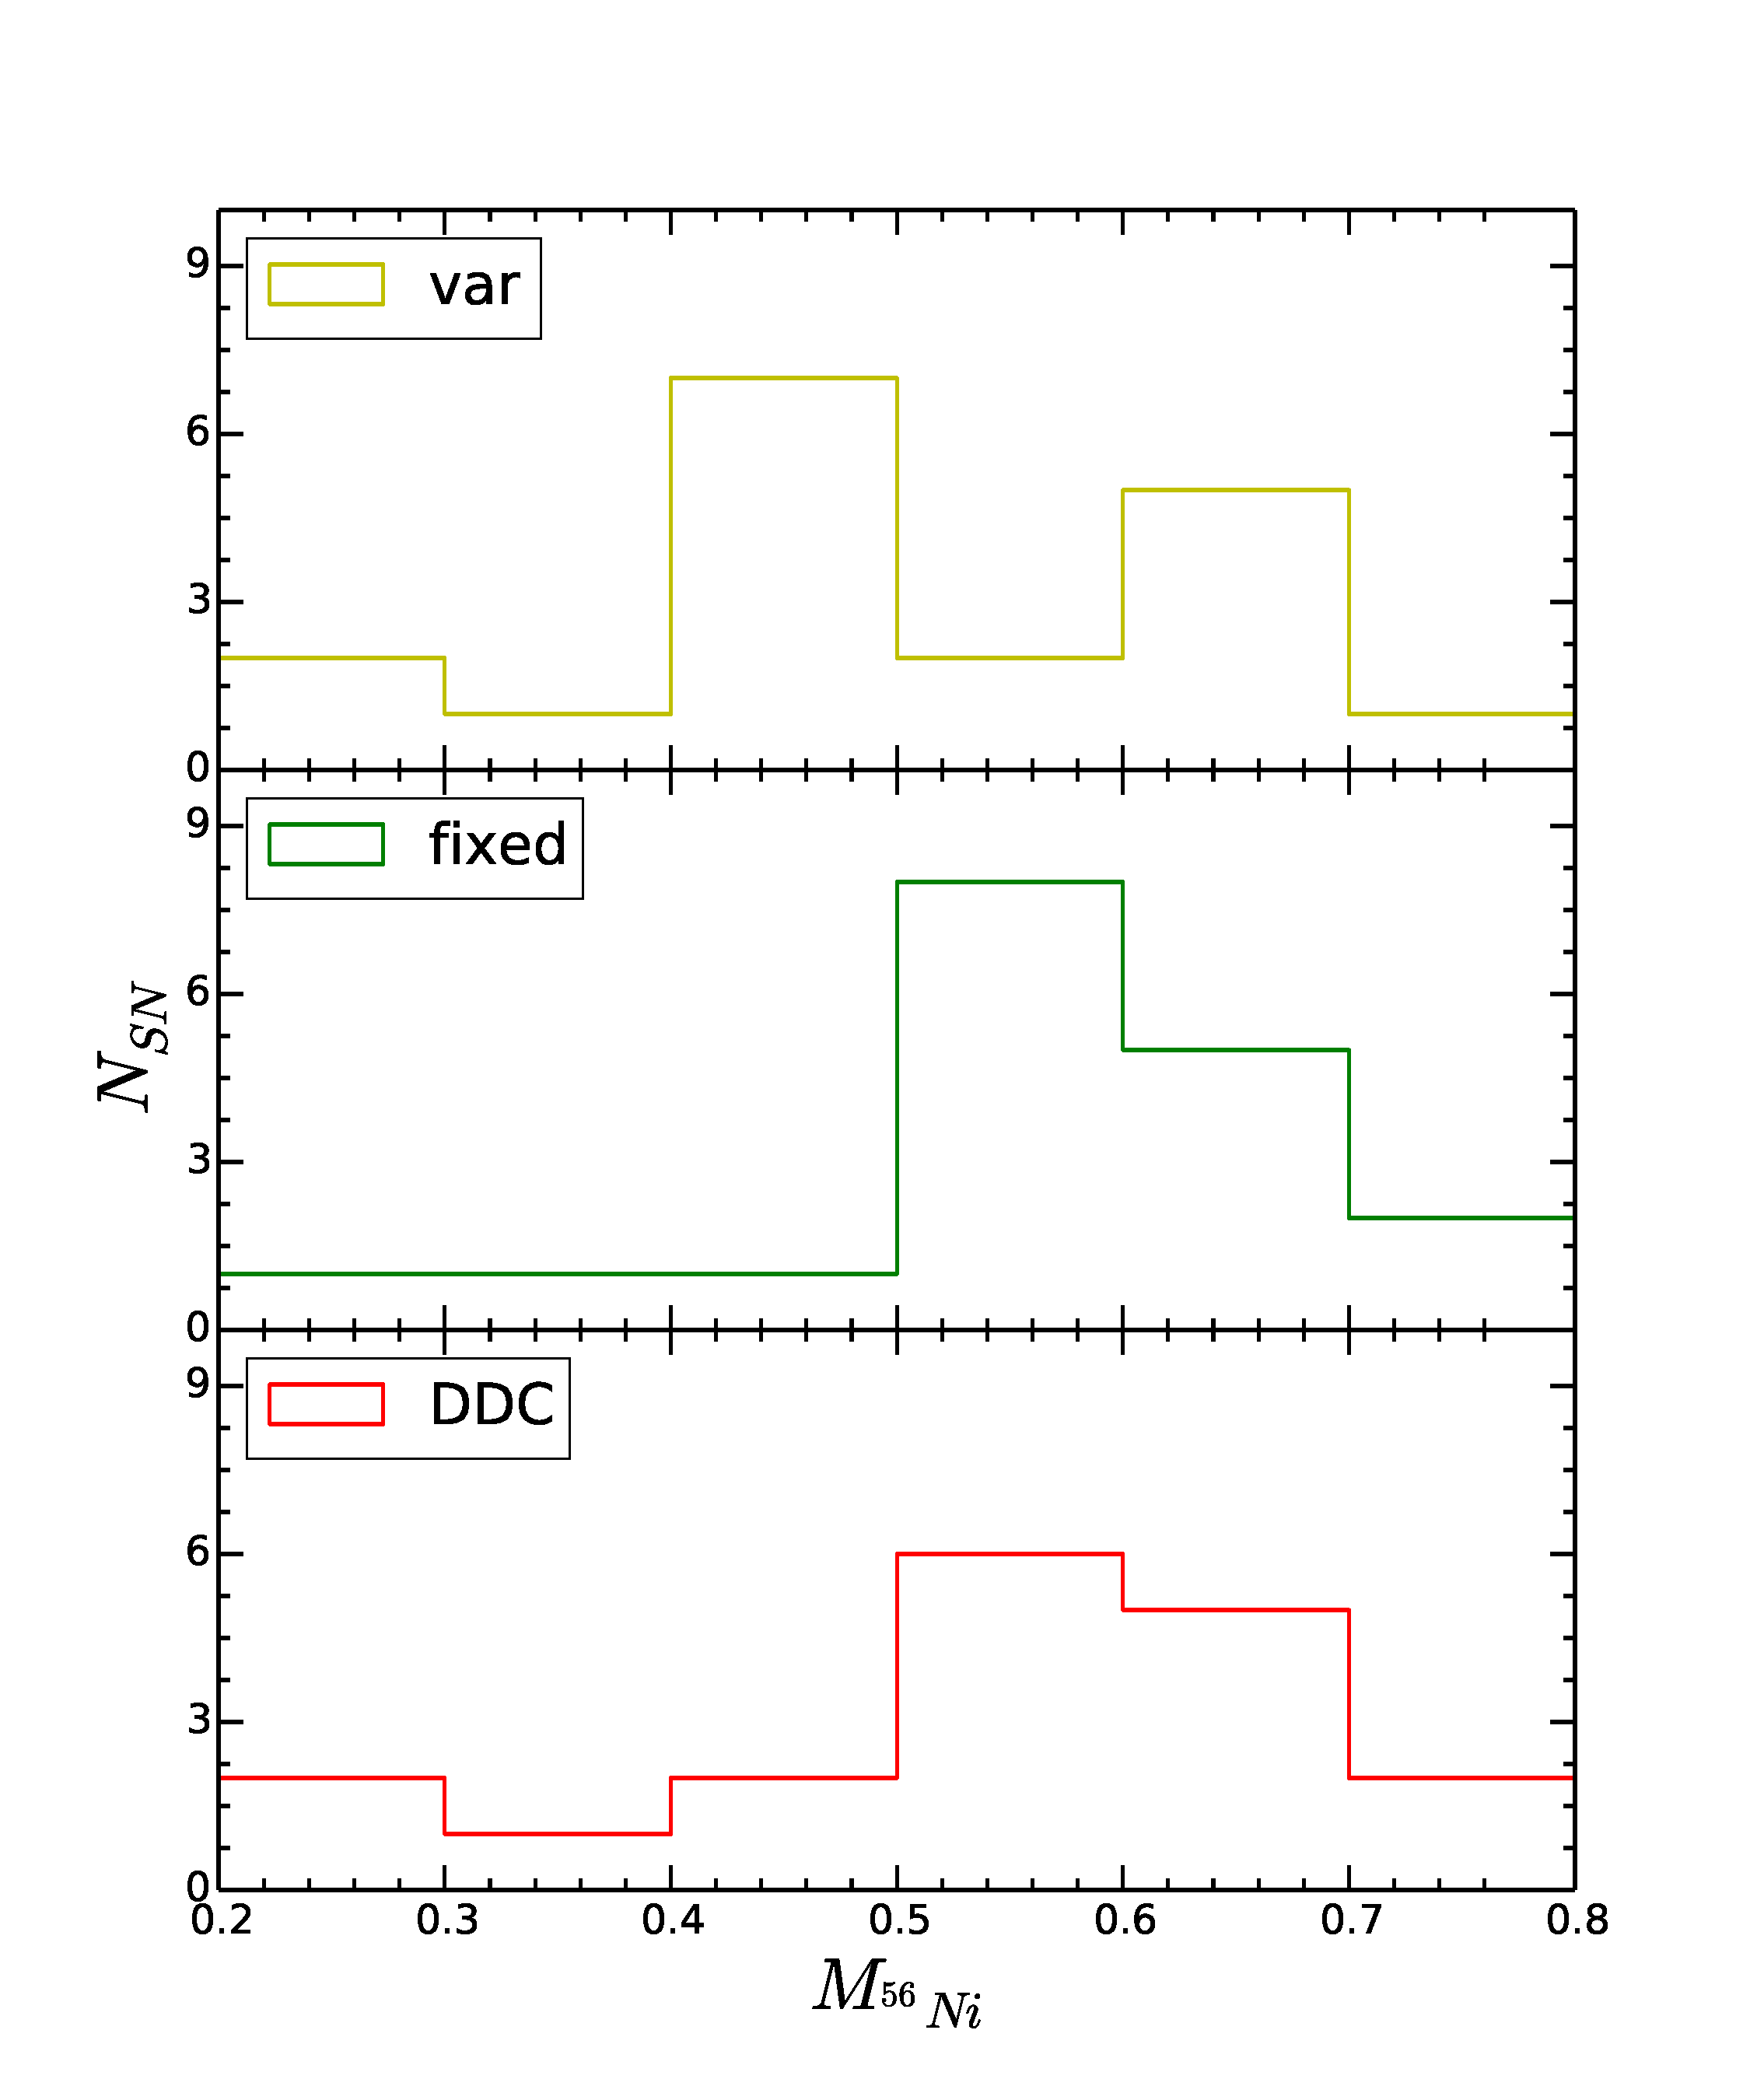
\includegraphics[width=.5\textwidth, trim= 0 30 0 30]{../plot_rel/hist_ni.pdf}
\caption{The histograms show the different methods to estimate the $M_{^{56}Ni}$ from the $L_{max}$. The values from Arnett's rule with fixed and variable rise time are plotted in the \emph{top} and \emph{middle} panels. The \emph{bottom} panel has the values estimated from the DDC models}
\label{fig:nicomp}
\end{figure}


Similar to previous studies we find that there is a large distribution in the $M_{^{56}Ni}$ values for the sample in Table \ref{tab:lr}. We note a factor of $\sim$ 3 difference between the lowest and highest $M_{^{56}Ni}$ values. We note that this sample doesn't include faint, 91bg-like objects, since their NIR light curves don't show a second maximum. These objects are seen to have a much lower $M_{^{56}Ni}$ $\sim$ 0.1 $M_{\odot}$. Thus, the complete distribution of $M_{^{56}Ni}$ for SNIa is expected to be wider than is seen in our sample.

%------------%


\subsection{Test Case for heavily reddened SNe}
Using the correlations derived above, we want to estimate the Ni masses of heavily reddened SNae. The first test case is the nearby SN 2014J in M82 with an $E(B-V)_{host}$ of 1.3. 
Current attempts to use the bolometric light curve depend on the $A_V$ value used and vary by a factor of $\sim$ 2
 (0.37 $M_{\odot}$ if using $A_V$=1.7 mag from \citet{Margutti2014}, compared to 0.77 using a higher $A_V$ of 2.5 mag from \citet{Goobar2014}).  In our analyses the aim is to 
 estimate the $M_{^{56}Ni}$ independent of the extinction.

The proximity of SN2014J, has allowed for the first $\gamma$ ray Co line detection in an SNIa (Churazov+ 2014). the authors, using a line photon escape fraction from the models, 
deduce an Ni mass of 0.62  $\pm$ 0.13 $M_{\odot}$. This provides a direct measurement of  $M_{^{56}Ni}$ for the SN. However, $\gamma$ ray detections aren't possible for farther away SN, for which we require a different estimation method. 

Using the best fit relation for the sample defined above , we obtain $M_{^{56}Ni}$ of 0.66 $\pm$ 0.15 $M_{\odot}$  for a $t_2$ of 31.99 $\pm$ 1.15 days. 
Thus, we find a very good correspondence between the values from the $\gamma$ rays and the NIR second maximum. This adds evidence to the argument that the NIR can be used for estimate $M_{^{56}Ni}$ for highly reddened SN.

Since we find from the DDC models that $\alpha$ is not constant for different $M_{^{56}Ni}$ (and hence, $L_{max}$) values, we use $\alpha$ corresponding to the peak luminosity of SN2014J. We do not find a significant change in the estimated $M_{^{56}Ni}$. Hence, for further analyses, we use $\alpha$=1

\begin{table*}
\begin{center}
\caption{Comparison of different methods to estimate $M_{^{56}Ni}$ for SN2014J}
\begin{tabular}{llcrr}
\hline
 $M_{Ni}$ (inferred) & $\sigma$ & Method & Reference\\
\hline
0.62	& 0.13 & $\gamma$ ray lines & \citet{Churazov2014} \\
0.37	& -- & Bolometric light curve $A_V$=1.7 mag &  \citet{Churazov2014, Margutti2014} \\
0.77	& -- & Bolometric light curve $A_V$=2.5 mag & \citet{Churazov2014, Goobar2014} \\
0.64	& 0.12 & NIR second maximum & this work \\

\hline
\end{tabular}
\end{center}
\label{tab:meth}
\end{table*}


For SN2014J, we can get a precise measurement of the extinction from IR spectra at $\sim$ +300 days ({\bf explain in greater detail}). This is again not possible for 
objects farther away. Thus, we apply this relation to a farther away, heavily extinguished object, SN2006X. 
The measured value for SN2006X of $t_2(J)$ is 28.19 with an error of 0.49  days. This results in an $M_{^{56}Ni}$ value of 0.58 $\pm$ 0.13 $M_{\odot}$. This value is consistent with the conclusion that SN2006X is a 'normal' SNIa \citep{Wang2008}. We compare this value for SN2006X to that obtained using $t_2(Y)$ and obtain $M_{^{56}Ni}$ of 0.58 $\pm$ 0.14 $M_{\odot}$. We find both these values consistent with each other. The slightly higher error bar on
 the value from $t_2(Y)$ is due to a larger error on the 
intercept in the best fit relation for the $Y$ band. 


In \citet{Wang2008}, the authors use multi-band photometry to correct the light curves for absorption from host galaxy dust. They derive a bolometric peak luminosity of 1.02 ($\pm$ 0.1) $\cdot e43$ $erg s^{-1}$. From $R$ band photometry, they derive a rise time to $B$ maximum of 18.2 $\pm$ 0.9d. Using this value in the expression for Arnett's rule, they derive a value of $M_{^{56}Ni}$= 0.50 $\pm$ 0.05 $M_{\odot}$. Thus, we conclude that the value derived from $t_2$ is consistent with published  $M_{^{56}Ni}$ values.   


\begin{table*}



\begin{center}
\caption{$M_{Ni}$ estimates for 5 objects with high values of $E(B-V)_{host}$. We present constraints from the relation using only $t_2(J)$ as well as from both $t_2(Y)$ and $t_2(J)$. We can see a marked decrease in the error values when combined constraints are used}
\begin{tabular}{llcccrr}
\hline
SN & $t_2(J)$ & $M_{Ni}$ (inferred) & $\sigma$ & $\mu$ & $e_{\mu}$ & Method \\
\hline
SN1986G	& 16.40 ($\pm$ 1.4)	&	0.32 & 0.10	& 28.01 & 0.12 & $J$ band relation \\
-- & --	& 0.33	& 0.08	&--&--& combined fit \\
SN2005A	& 27.58 ($\pm$ 0.3)	& 0.57	&  0.13 & 34.51 & 0.11  & $J$ band relation \\
-- & -- &	0.57	& 0.11	&--&--& combined fit \\
SN2006X	& 28.19  ($\pm$ 0.5)	& 0.57 & 0.13 &	 30.91 & 0.08 & $J$ band relation \\
-- & -- &	0.58	& 0.11	&--&--& combined fit \\
SN2008fp & 31.03 ($\pm$ 0.3)	& 0.64	& 0.15 & 31.79 & 0.05 & $J$ band relation \\
-- 	- &-- & 0.64	& 0.13	&--&--& combined fit		\\
SN2014J	& 31.99 ($\pm$ 1.2)	& 0.66	& 0.15 &  27.64 & 0.10   & $J$ band relation\\
--	& -- & 0.66  & 0.13 &--&--& combined fit \\
\hline
\end{tabular}

\label{tab:red}

\end{center}




\end{table*}



We include three more objects in the highly reddened SNe sample, namely, 1986G, 2005A and 2008fp. We calculate the $M_{^{56}Ni}$ for these objects in the same way as for SN2014J and SN2006X. We summarise our findings in Table ~\ref{tab:red}.
We can see that 1986G has a lower value of $M_{^{56}Ni}$ than the other objects in the sample. This is consistent with the observed optical decline rate and lower $B$ band luminosity of the SN. Since we find that $t_2$ in both $Y$ and $J$ bands correlates very strongly with the $M_{^{56}Ni}$, we use combined constraints from the relations to obtain an $M_{^{56}Ni}$ estimate.

% We can see from Table ~\ref{tab:red} that the error on the $M_{^{56}Ni}$ reduces when using combined constraints. For 2014J, it is 0.17 $M_{\odot}$ whereas for the others it is much lower at 0.07 $M_{\odot}$ 


Hence, we conclude that the NIR second maximum timing (in $Y$ and $J$) is a very good indicator of the amount of Nickel synthesised in the explosion, even for heavily reddened objects. 


\subsubsection{Combined fit}
From our analyses, we've found that the $t_2$ in $Y$ and $J$ is very strongly correlated to the $L_{max}$. In table \ref{tab:coeff}, we see that the slope values for the two bands is nearly identical and the intercepts are within the error bars. This prompted us to combine the information from the two bands for extrapolating the values of $L_{max}$ for objects not in the 'low-reddening' sample.

For the five objects listed above which have a very high $A_V$, we used the $J$ band relation to obtain an $M_{^{56}Ni}$. We also used a combined fit to the $Y$ and $J$ band data to evaluate the reduction in the error bar. For this, we presume that the $Y$ band estimate is equivalent to the value in the $J$ band, and hence, we calculate the slope and intercept with a greater number of data points, which leads to a reduction in the errors on the parameter estimates.  

\subsection{Complete NIR Sample}
Since we have derived the relation between $L_{max}$ and $t_2$, we evaluate the $L_{max}$ for all objects with a measured $t_2$ independent of the reddening estimates.
Since the slope for the relation in the $Y$ and $J$ bands is very similar and the intercepts are within error bars, we take the mean value for the slope and intercepFt as a 'combined' relation. We use the higher error on the intercept (from the $Y$ band) for the combined equation. We then use this to compare the estimates of $L_{max}$ from the $t_2$ in the two bands. In figure \ref{fig:yjcomp}, we plot the difference in the $L_{max}$ from the $t_2$ in $J$ and $Y$ against the $L_{max}$ estimated from $t_2(J)$. The difference in the two estimates is smaller than the error on the measurement. We note that the largest difference is for SN2005na, which has a $t_2(J)$ of 32.59, but a much smaller $t_2(Y)$ of 27.54. However, even for this object, the error is higher than the difference between the measurements   
%and have presented the different ways to obtain the $M_{Ni}$ from the $L_{max}$, we can then use the distribution of $t_2$ for all objects, independent of reddening to obtain a distribution of $M_{^{56}Ni}$ using the relations derived


\begin{figure}
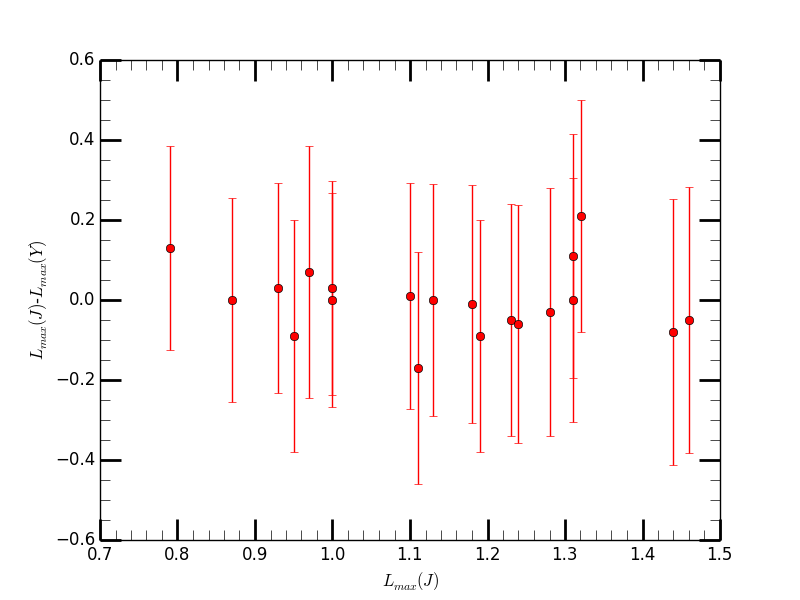
\includegraphics[width=.5\textwidth, height=0.25\textheight, trim= 0 30 0 30]{../plot_rel/lbol_comp_yj.png}


\caption{A comparison of the $L_{max}$ from the $t_2$ values measured in the $Y$ and $J$ bands. Plotted on the x-axis is the $L_{max}$ measured from $t_2(J)$ and on the y-axis is the difference between $L_{max}(J)$ and $L_{max}(Y)$. We can see that there is no trend between the two. The difference has a standard deviation of 0.08 ($\cdot$ $1e^{43}$) $erg s^{-1}$. The errors on each are errors in the individual measurements added in quadrature. We can see that the difference is smaller than the error. }
\label{fig:yjcomp}
\end{figure}

In section \ref{ssec-derni}, we have described the different methods for obtaining $M_{^{56}Ni}$ from $L_{max}$. Hence, we can derive a distribution for $M_{^{56}Ni}$ from the evaluated $L_{max}$ for the complete sample. 
\begin{figure}
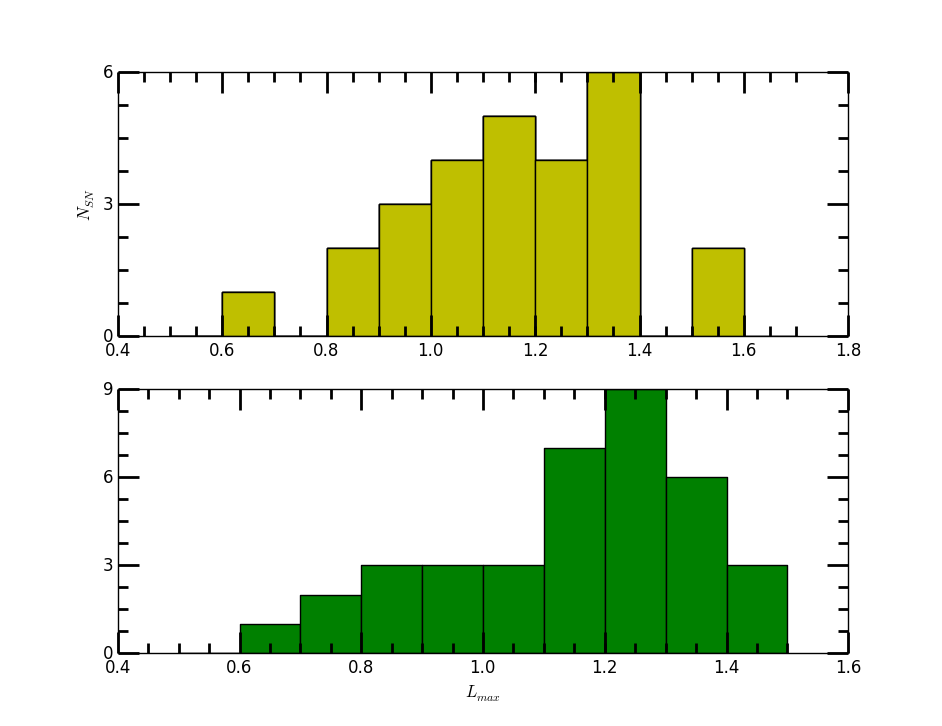
\includegraphics[width=.5\textwidth, trim= 0 30 0 30]{../plot_rel/lbol_yj_compsamp.png}
\caption{Histogram distributions of $L_{max}$ derived from the relations for the complete sample of objects (without the low reddening sample). \emph{Top}: Using the $t_2(Y)$ and \emph{bottom}: Using the $t_2(J)$. A large distribution in the $L_{max}$ values can be seen}
\label{fig:hist}
\end{figure}


In figure \ref{fig:hist} we plot the distribution of $M_{^{56}Ni}$ calculated from the $L_{max}$. We use Arnett's rule with a fixed rise time to get the $M_{^{56}Ni}$ from the $L_{max}$. From figure \ref{fig:hist}, we find a large scatter in the $M_{^{56}Ni}$ values. We find that the objects vary by a factor of 3 in their $M_{^{56}Ni}$ distribution. We note, however, that since faint, 91bg-like objects do not show a second maximum, we do not have values in the figure $\lesssim$ 0.2 $M_{\odot}$, hence, the expected variation for the complete population of SNIa is greater.  


\begin{table}
\begin{minipage}{70mm}
\begin{center}
\footnotetext{$^a$:$\cdot e^{43} erg s^{-1}$}
\caption{$M_{Ni}$ measurements for the complete sample of objects with $t_2$ measurements in both $Y$ and $J$ bands.}
\begin{tabular}{llcrr}
\hline
SN & $L_{max}^{a}$ (J)	& $\sigma$ & $L_{max}^{a}$ (Y) & $\sigma$ \\
\hline
1980N & 0.91 & 0.13 &\ldots & \ldots \\
1981B & 1.32 & 0.15 &\ldots & \ldots\\
1986G & 0.64 & 0.09 &\ldots & \ldots\\
1998bu & 1.23 & 0.14 &\ldots & \ldots\\
1999ac & 1.12 & 0.14 &\ldots & \ldots\\
1999ee & 1.42 & 0.16 &\ldots & \ldots \\
2000E & 1.31 & 0.16 &\ldots & \ldots\\
2000bh & 1.37 & 0.15 &\ldots & \ldots\\
2001bt & 1.17 & 0.13 &\ldots & \ldots\\
2001cn & 1.24 & 0.14 &\ldots & \ldots\\
2001cz & 1.40 & 0.16 &\ldots & \ldots\\
2001el & 1.29 & 0.15 &\ldots & \ldots\\
2002bo & 1.12 & 0.13 &\ldots & \ldots\\
2003cg & 1.24 & 0.14 &\ldots & \ldots\\
2003hv & 0.92 & 0.12 &\ldots & \ldots \\
2004ey	&	1.21	&	0.19	&	1.31	&	0.20	\\
2004gs	&	0.93	&	0.16	&	0.91	&	0.16	\\
2004gu	&	1.46	&	0.22	&	1.54	&	0.22	\\
2005A	&	1.10	&	0.18	&	1.12	&	0.18	\\
2005al	&	1.05	&	0.18	&	1.04	&	0.18	\\
2005na	&	1.35	&	0.20	&	1.13	&	0.19	\\
2006D	&	1.05	&	0.18	&	1.01	&	0.18	\\
2006X	&	1.13	&	0.18	&	1.13	&	0.19	\\
2006ax	&	1.32	&	0.20	&	1.36	&	0.21	\\

2006et	&	1.33	&	0.22	&	1.35	&	0.20	\\
2006gt 	& 0.85 		& 0.11 &\ldots & \ldots\\
2006hb	&	0.79	&	0.17	&	0.72	&	0.15	\\
2006kf	&	1.01	&	0.17	&	1.07	&	0.10	\\
2007S	&	1.46	&	0.21	&	1.52	&	0.23	\\
2007af	&	1.22	&	0.19	&	1.23	&	0.19	\\
2007as	&	1.02	&	0.22	&	0.94	&	0.17	\\
2007bc  &\ldots & \ldots & 1.16 &  0.2 \\
2007bm	&	1.15	&	0.17	&	1.32	&	0.20	\\
2007ca  &\ldots & \ldots & 1.38 &  0.22 \\
2007if  &\ldots & \ldots & 1.34 & 0.22 \\
2007jg  &\ldots & \ldots & 1.12 & 0.2  \\
2007le	&	1.27	&	0.20	&	1.31	&	0.20	\\
2007nq	&	0.98	&	0.18	&	0.94	&	0.17	\\
2008C	&	1.33	&	0.21	&	1.23	&	0.19	\\
2008fp	&	1.28	&	0.20	&	1.33	&	0.21	\\
2014J & 1.32 & 0.18 &\ldots & \ldots \\
\hline
\end{tabular}
\end{center}
\end{minipage}
\label{tab:yj}
\end{table}


In table \ref{tab:comp_ni}, we present the  $M_{^{56}Ni}$ values for the complete sample of objects with a measured $t_2(J)$ value. 




\iffalse
\begin{figure}
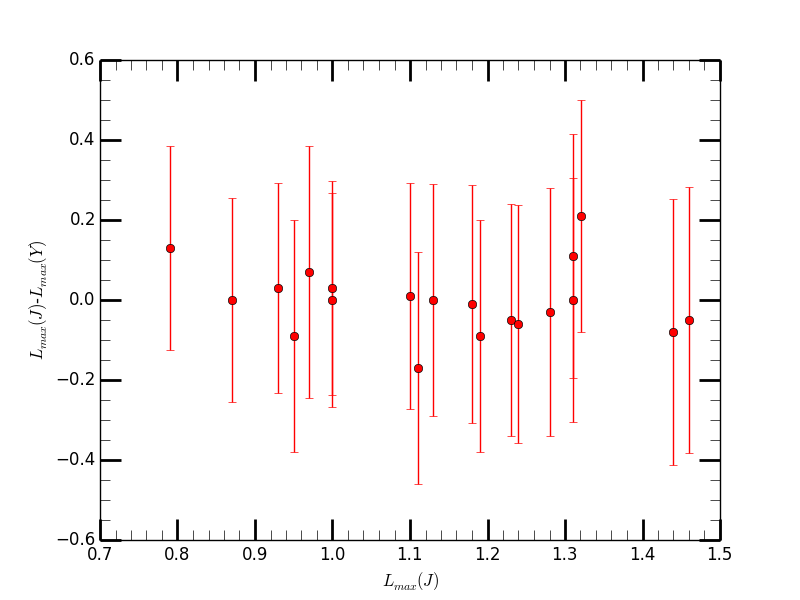
\includegraphics[width=.5\textwidth, trim= 0 30 0 30]{../plot_rel/lbol_comp_yj.pdf}
\caption{The plot shows the difference in the $M_{^{56}Ni}$ measured using $Y$ and $J$ band data, plotted against the $M_{^{56}Ni}$ measured from the $J$ band data. The mean value of the difference is 0.03 $M_{\odot}$ with a standard deviation of 0.037 $M_{\odot}$ (error bars on the x-axis have not been plotted for better visibilty of points)}
\label{fig:yjcomp}
\end{figure}
\fi

In figure \ref{fig:yjcomp}, we plot the difference between the $L_{max}$ estimated from the $t_2$ in $Y$ and $J$ bands against the $L_{max}$ estimated from $t_2(J)$ (called $L_{max}(J)$ in the figure). We find that there is no relation between the two quantities. The mean difference is 0.06 $M_{\odot}$ with a standard deviation of 0.05 $M_{\odot}$. This is lower than the error estimate on the individual values, which can be seen in the figure. 	


\subsection{Comparison with published values}
We searched the literature for published values of $M_{^{56}Ni}$ for objects in our sample. In \citet{Scalzo2014} , the authors published values of $M_{^{56}Ni}$ for 2005el and 2011fe. For 2011fe, we find $M_{^{56}Ni}$ of 0.52 $\pm$ 0.15 $M_{\odot}$ whereas the value in S14 is 0.42 $\pm$ 0.08. We note that the value of $\alpha$ in their study is 1.2 whereas we use $\alpha$=1. Using their value of $\alpha$, we find $M_{^{56}Ni}$= 0.44 $M_{\odot}$, which is a better agreement. SN2011fe also has a publsihed $M_{^{56}Ni}$ value in \cite{Pereira2013}, where the authors use different values of $\alpha$. For $\alpha$=1 they report a value of 0.53 $\pm$ 0.11 $M_{\odot}$, which agrees well with the value in this work. 

For SN2005el we find $M_{^{56}Ni}$ of 0.46 $\pm$ 0.11 $M_{\odot}$. S14 provides a discussion of this object, which in their sample they measure to have an  $M_{^{56}Ni}$ of 0.52. It is one of two outliers in their $M_{^{56}Ni}$-$\Delta m_{15}$. They argue that it is likely for the SN to have a lower $M_{^{56}Ni}$ that their fiducial analysis suggests.  




























